\section{Methods}

Here I describe the two environments and the behaviors that we are targeting within them. 

\subsection{The patch harvesting environment}

% What are we modeling?
The first environment aims to model the patch harvesting behavior of early bilaterians as they traversed microbial mats. 
Fossil records of the paths taken by these animals provide evidence of complex behavioral patterns, potentially resulting from early cognitive behaviors \citep{carboneWhenLifeGot2014}. 
This environment is a re-implementation of the one found in \citep{pontesEvolutionaryOriginsCognition2021}. 
In this environment, organisms are rewarded for consuming nutrients and punished for time spent off the patch. 
Here, we specifically look at environments with multiple patches of nutrients, and our target behavior is the successful consumption of multiple patches. 
This behavior requires switching between at least two tasks (exploring or exploiting), and as such, it is a cognitive behavior comparable to associative learning in Chapter \ref{chap:replaying_associative_learning}.
%This behavior requires memory to solve, and as such it presents a testbed for a cognitive behavior that is comparable to associative learning in previous work. 
%aim to quantify the potentiation of memory usage required to switch between exploiting one patch and exploring to find a new patch. 

% General overview of how the environment is used
Our Avida organisms exist in the typical 60x60 toroidal grid, with parent organisms replicating into a neighboring cell. 
The evaluation of the organisms, however, occurs on a toroidal, two-dimenstional spatial grid that represents microbial mats like those encountered by the early bilaterians. 
These environments consist of various patterns of nutrients that the organisms can consume and empty tiles whose traversal causes the organisms to waste energy. 

% How does the environment actually work?
To facilitate the consumption of nutrients, organisms are granted four new instructions to navigate their environment. 
Movement is accomplished via three instructions: \texttt{Turn Left}, \texttt{Turn Right}, and \texttt{Move Forward}. 
The right and left instructions rotate the organism 45 degrees in the appropriate direction. 
The move instruction always moves the organism a single tile in the direction it is pointing, including diagonally. 
Finally, the organisms are given a \texttt{Sense} instruction to pull information from their environment. 
Specifically, the sense instruction will give the organism a numeric cue depending on what floor tile it is currently on. 
%Nutrient tiles result in a 3 cue, while 
Empty tiles return a negative one, while already-consumed nutrient tiles result in positive one. 
Nutrients are consumed as the organism moves onto that tile without requiring an additional action, and as such organisms will never sense a nutrient tile that has not been consumed.  

% How does scoring work? 
Organisms are scored based on how well they consume nutrients and avoid empty tiles. 
The organism's score is increased by one for each nutrient consumed. 
For every empty tile visited, however, the organism's score is reduced by one to model the organism expending energy to move for no nutrient gain. 
Moving onto a previously-consumed tile has no effect on score, as if some residual nutrients could offset the energy consumption. 
Finally, as is often done in Avida, this score is used in an exponential. 
The performance of the organism is calculated as $2^{\text{score}}$, which means an additional nutrient consumed always doubles performance, regardless of how many nutrients have been consumed in total. 
As is customary in Avida, this score is used to weight which organisms receive the most updates and thus execute their genomes faster. 

\begin{figure}
    \centering
    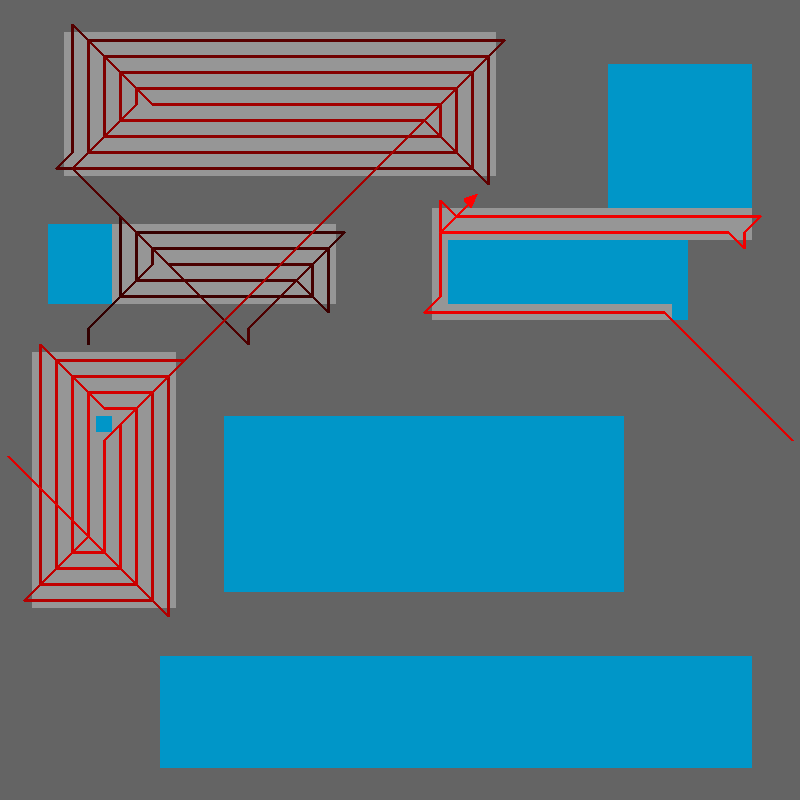
\includegraphics[width=0.9\textwidth]{06_memory_in_patch_harvesting/media/patch_harvest_example.png}
    \caption{
    An example layout of disconnected patches in the patch harvesting environment.
    Blue tiles represent food that has yet to be consumed, light gray tile are food that has been consumed, and dark gray tiles show empty space which is costly to move into. 
    The lines show the trace of an evolved organism (red triangle), with the start of the line in black and a slow fade to red as the trace becomes more recent. 
    This organism has evolved a spiraling behavior and has successfully consumed three patches of food. 
    }
    \label{fig:patch_harvest:example}
\end{figure}

% For more example images, see seeds 27, 31, and 32 for disconnected patches without edges

% Discussion of the target behavior and why it's cool
While previous work has used multiple patch types \citep{pontesEvolutionaryOriginsCognition2021}, here I propose to study only one: multiple disconnected patches.
The smaller patches in this environment require organisms to switch patches once they have exploited their current patch in order to maximize their score. 
These two behaviors (exploration and exploitation) can be thought of as two states the organism can be in.
As such, I expect this behavior to require memory, as a single bit of information is needed to store what state the organism is in. 
% The organism must determine when it has successfully consumed a patch and then move to find a new patch to eat. 
% This requires at least two states of behavior. 
Figure \ref{fig:patch_harvest:example} shows an example of the disconnected patches, as well as an evolved organism's successful trace through the environment. 
To easily categorize organisms that are capable of consuming multiple patches, I will require the organism to have consumed at least half each of two patches to be considered a ''successful'' behavior. 
Exploratory work has shown that this behavior does evolve, but only rarely. 
In 200 initial replicates, it appeared in only nine. % replicates. 
%This rarity works in our favor, as rare behaviors have the most room for potentiation gain. 
Much like associative learning in previous work, this rarity provides substantial room for improvements in potentiation over the course of a lineage. 

\subsection{The cyclic logic 6 environment}

% Intro
There may be inherent similarities between the associative learning task of Chapters \ref{chap:alife_submission} and \ref{chap:replaying_associative_learning} and the cognitive behavior needed in the patch harvesting environment. 
As such, here I propose one final, non-cognitive environment to test potentiation: the cyclic environment from Chapter \ref{chap:consequences_of_plasticity}, which I will refer to here as ``cyclic logic 6''. 

% Overview of environment
The cyclic logic 6 environment in Avida consists of two sets of bitwise logic tasks: one that is rewarded and one that is punished. 
Which set is rewarded, however, switches at regular intervals. 
Each organism receives a set of random input numbers, and then has the opportunity to perform computations and eventually output these values.  %performs whatever computation on them, and potentially outputs one or more values. 
If output values are deemed to be a successful logic operation on one or more inputs, then the organism is rewarded or punished according to the current state of the environment.  
The Avida organisms, however, are only given access to a bitwise \texttt{NAND} instruction, which they must use to build the other logic operations. 
% The simplest two tasks, NOT and NAND, confer a reward of 2, while we increase to a reward of 4 for AND and ORNOT, 8 for ANDNOT and OR, 16 for XOR and NOR, and finally a reward of 32 for EQU. 
% Rewards are multiplicative, so performing NOT and XOR would result in a performance of 32. 
% Organisms are only rewarded once for each logic task they perform. 

% Explanation of cycling
At any given time, three of the six logic tasks will be rewarded while the other three are punished. 
In this cyclic environment, this reward scheme is flipped at regular intervals.
%When this flip occurs, tasks that were rewarded become punished and vice versa. 
%An organism's score is doubled when it performs a rewarded task for the first time and halved when performing a punished task for the first time. 
When performing a logic task for the first time, an organism's score is doubled if that task is rewarded or halved if the task is punished. 
Here I flip the rewards and punishments every 100 updates. 
I will give organisms access to a new instruction, \texttt{Sense}, so they can determine what environment they are in and can potentially regulate task expression accordingly.
This environment is described in detail in Chapter \ref{chap:consequences_of_plasticity}, though here I am only using the PLASTIC environment from Phase 1 (see Figure \ref{fig:experimental-design}, panels A and C). 
I will use the same two sets of tasks used in Chapter \ref{chap:consequences_of_plasticity} (NOT, AND, and OR) and (NAND, AND-NOT, OR-NOT).

% What is optimal plasticity?
Due to the cycling of which tasks are rewarded, organisms must exhibit optimal plasticity to maximize fitness. 
As in the previous chapter, I define optimal plasticity as performing the three rewarded tasks and zero of the punished tasks. 
While organisms are born into a particular environment, I will test for optimal plasticity \textit{post hoc}, evaluating the organism in both variations of the environment. 
Therefore, for an organism to exhibit optimal plasticity, they must be capable of perfectly regulating all six tasks depending on which environment they are in. 

% Optimal plasticity is our target behavior
It is this optimal plasticity that I will target for the potentiation analysis. 
Compared to associative learning and multi-patch harvesting behaviors, optimal plasticity is a much more common behavior to evolve from the ancestor, with Chapter \ref{chap:consequences_of_plasticity} seeing greater than 40\% of replicates evolve the behavior.
While it is may be more common, this behavior is still nontrivial. 
To perform optimal plasticity, organisms must be capable of performing all six logic tasks, sensing the environment, and using the environment data to regulate the execution of the logic tasks. 
This task, however, can be solved reactively; it is unnecessary to store the environment state in memory. 
Still, I expect the complex nature of the environment to translate into interesting patterns in potentiation, not unlike those of associative learning seen in previous work. 



% Logic 9 has been well-studied in Avida. 
% Previous work has looked into how different evolutionary dynamics factor into the evolutionary dynamics of the more complex logic tasks, specifically equals (EQU) [CITE]. 
% As such, EQU provides us with a difficult-to-evolve target behavior that we can use for our potentiation studies. 
% By running analytic replays on lineages that evolve EQU, we can see how their likelihood to evolve the behavior changed over time. 
% This behavior has the potential to be quite different from associative learning from previous chapters or memory usage in the previous environment, as EQU does not require any cognitive processes. 
% Thus, the potentiation of EQU will be a solid basis of comparison as a behavior that does not require memory but is still difficult to evolve. 